\chapter{Analisi}
In questo capitolo sono riportati i risultati e i tempi ottenuti per ogni fase: dalle procedure ETL all'esecuzione delle query.

\section{Prestazioni ETL}
\subsection{Trasformazione in CSV}
In questa sezione copriremo un'analisi dei tempi ottenuti nella fase che permette, a partire dai dati originali, di ottenere un file in formato CSV contenente i dati ripuliti da inconsistenze e in un formato adatto ad essere importato nel Datawarehouse.
In particolare nella fase di puliza, a partire dal file XSLX, si estraggono unicamente i record dove non appaiono valori negativi per quantità intrinsecamente positive (concentrazione, volume, ecc.); per i record ove manca il valore "relative" e/o la distanza percorsa si procede ad un calcolo a partire dall'ultima rilevazione valida estratta. Inoltre tutte le righe che presentano una chiara assenza di dati (70\% delle colonne) vengono scartate. Infine, durante la fase di trasformazione, per ogni file viene generata una data e un test\_id e per separare la parte intera da quella decimale si sostituisce la virgola con il punto.\\
I dati ottenuti si riferiscono ad una media aritmetica ottenuta testando 200 file ($\sim$1 milione di righe) generati a partire dal file originario fornito dall'Istituto Motori di Napoli.

\begin{table}[H]
	\centering
\begin{tabular}{ccccc}
	\rowcolor[HTML]{333333} 
	{\color[HTML]{FFFFFF}Righe XSLX}  
	& 
	{\color[HTML]{FFFFFF}Righe CSV}
	&
	{\color[HTML]{FFFFFF}Righe perse}
	&
	{\color[HTML]{FFFFFF}Peso file XSLX}
	&                                 
	{\color[HTML]{FFFFFF}Peso file CSV}\\
	\begin{tabular}[c]{@{}l@{}}5764\end{tabular}             
	& \begin{tabular}[c]{@{}l@{}}5706\end{tabular} 
	& \begin{tabular}[c]{@{}l@{}}1\%\end{tabular}  
	& \begin{tabular}[c]{@{}l@{}}2.138KB\end{tabular}  
	& \begin{tabular}[c]{@{}l@{}}2.283KB\end{tabular}   
\end{tabular}
\end{table}

\begin{table}[H]
	\centering
	\begin{tabular}{ccc}
		\rowcolor[HTML]{333333} 
	{\color[HTML]{FFFFFF}Fase di pulizia}
	&
	{\color[HTML]{FFFFFF}Fase di trasformazione}
	&
	{\color[HTML]{FFFFFF}Tempo totale}\\
	\begin{tabular}[c]{@{}l@{}}3.04s\end{tabular}             
	& \begin{tabular}[c]{@{}l@{}}0,05s\end{tabular} 
	& \begin{tabular}[c]{@{}l@{}}3,05s\end{tabular}
\end{tabular}
\end{table}

\noindent{}Questa fase mette in luce la buona qualità dei dati forniti dall'istituto: ci si aspetta in media di perdere pochissimi dati a causa di inconsistenze. Per quanto riguarda invece le dimensioni si nota come il formato Comma-separated values sia leggermente meno efficiente nella compressione rispetto al formato proprietario di Microsoft$^{\tiny{\textregistered}}$ ma al tempo stesso permetta una più veloce elaborazione.

\subsection{Import in Tabella Temporanea}
Al fine di importare i file CSV nella tabella dei fatti ci si appoggia ad una tabella temporanea al fine di agevolare le operazioni successive. Questa tabella viene troncata alla fine della procedura. L'import sfrutta la funzione \textit{COPY} messa a disposizione dal DBMS PostgreSQL.

\begin{table}[H]
	\centering
	\begin{tabular}{ccc}
		\rowcolor[HTML]{333333} 
		{\color[HTML]{FFFFFF}Numero file}
		&
		{\color[HTML]{FFFFFF}Numero righe}
		&
		{\color[HTML]{FFFFFF}Tempo}\\
		\begin{tabular}[c]{@{}l@{}}1\end{tabular}             
		& \begin{tabular}[c]{@{}l@{}}5706\end{tabular} 
		& \begin{tabular}[c]{@{}l@{}}214ms\end{tabular}\\
		\rowcolor[HTML]{C0C0C0}
		\begin{tabular}[c]{@{}l@{}}50\end{tabular}             
		& \begin{tabular}[c]{@{}l@{}}285.300\end{tabular} 
		& \begin{tabular}[c]{@{}l@{}}8,428s\end{tabular}\\
		\begin{tabular}[c]{@{}l@{}}100\end{tabular}             
		& \begin{tabular}[c]{@{}l@{}}570.600\end{tabular} 
		& \begin{tabular}[c]{@{}l@{}}16.522s\end{tabular}
	\end{tabular}
\caption{I dati si riferiscono ad una media di 5 esecuzioni}
\end{table}	
\noindent{}I risultati mostrano la bontà della funzione \textit{COPY} che sfruttando un inserimento batch di 1000 righe per volta riesce ad abbattere in modo consistente i tempi.

\subsection{Import nello Schema}
In questa fase i dati, precedentemente inseriti in una tabella temporanea, vengono travasati nello schema proposto dopo aver disabilitato tutti gli indici. Le prove effettuate prendono in considerazione diverse dimensioni della tabella dei fatti oltre al caso in cui lo schema risulti partizionato.
\begin{table}[H]
	\centering
	\begin{tabular}{cccc}
		\rowcolor[HTML]{333333} 
		{\color[HTML]{FFFFFF}Dimensione tab. fatti}
		&
		{\color[HTML]{FFFFFF}Numero righe importate}
		&
		{\color[HTML]{FFFFFF}Partizionamento}
		&
		{\color[HTML]{FFFFFF}Tempo}\\
		\begin{tabular}[c]{@{}l@{}}0\end{tabular}             
		& \begin{tabular}[c]{@{}l@{}}285.300\end{tabular} 
		& \begin{tabular}[c]{@{}l@{}}No\end{tabular}
		& \begin{tabular}[c]{@{}l@{}}3,925s\end{tabular}\\
		\rowcolor[HTML]{C0C0C0}
		\begin{tabular}[c]{@{}l@{}}0\end{tabular}             
		& \begin{tabular}[c]{@{}l@{}}285.300\end{tabular} 
		& \begin{tabular}[c]{@{}l@{}}Si\end{tabular}
		& \begin{tabular}[c]{@{}l@{}}7,753s\end{tabular}\\
		\begin{tabular}[c]{@{}l@{}}570.600\end{tabular}             
		& \begin{tabular}[c]{@{}l@{}}285.300\end{tabular} 
		& \begin{tabular}[c]{@{}l@{}}No\end{tabular}
		& \begin{tabular}[c]{@{}l@{}}3,730s\end{tabular}\\
		\rowcolor[HTML]{C0C0C0}
		\begin{tabular}[c]{@{}l@{}}570.600\end{tabular}             
		& \begin{tabular}[c]{@{}l@{}}285.300\end{tabular} 
		& \begin{tabular}[c]{@{}l@{}}Si\end{tabular}
		& \begin{tabular}[c]{@{}l@{}}7,404s\end{tabular}\\
		\begin{tabular}[c]{@{}l@{}}1.141.200\end{tabular}             
		& \begin{tabular}[c]{@{}l@{}}285.300\end{tabular} 
		& \begin{tabular}[c]{@{}l@{}}No\end{tabular}
		& \begin{tabular}[c]{@{}l@{}}4,535s\end{tabular}\\
		\rowcolor[HTML]{C0C0C0}
		\begin{tabular}[c]{@{}l@{}}1.141.200\end{tabular}             
		& \begin{tabular}[c]{@{}l@{}}285.300\end{tabular} 
		& \begin{tabular}[c]{@{}l@{}}Si\end{tabular}
		& \begin{tabular}[c]{@{}l@{}}8,572s\end{tabular}
		
	\end{tabular}
	\caption{I dati si riferiscono ad una media di 5 esecuzioni}
\end{table}	
\noindent{}Dalla tabella emerge come il partizionamento comporti quasi un raddoppio del tempo necessario all'inserimento: ciò è dovuto al dover spalmare un singolo record della tabella temporanea su 4 differenti tabelle. Questo slow-down è risolvibile pensando a 4 inserimenti in parallelo: infatti le 4 tabelle, anche se logicamente collegate, durante l'inserimento non necessitano di condividere alcuna informazione.

\subsection{Aggiornamento degli Indici}
In questa fase vengono riattivati gli indici delle chiavi tra tabella dei fatti e dimensioni. Questi indici sono assolutamente necessari per velocizzare le query ma possono essere disabilitati durante la fase di update dello schema.
\begin{table}[H]
	\centering
	\begin{tabular}{ccc}
		\rowcolor[HTML]{333333} 
		{\color[HTML]{FFFFFF}Dimensione tab. fatti}
		&
		{\color[HTML]{FFFFFF}Partizionamento}
		&
		{\color[HTML]{FFFFFF}Tempo}\\
		\begin{tabular}[c]{@{}l@{}}285.300\end{tabular}              
		& \begin{tabular}[c]{@{}l@{}}No\end{tabular}
		& \begin{tabular}[c]{@{}l@{}}2,530s\end{tabular}\\
		\rowcolor[HTML]{C0C0C0}
		\begin{tabular}[c]{@{}l@{}}285.300\end{tabular}              
		& \begin{tabular}[c]{@{}l@{}}Si\end{tabular}
		& \begin{tabular}[c]{@{}l@{}}11,534s\end{tabular}\\	\begin{tabular}[c]{@{}l@{}}570.600\end{tabular}              
		& \begin{tabular}[c]{@{}l@{}}No\end{tabular}
		& \begin{tabular}[c]{@{}l@{}}6,194s\end{tabular}\\
		\rowcolor[HTML]{C0C0C0}
		\begin{tabular}[c]{@{}l@{}}570.600\end{tabular}              
		& \begin{tabular}[c]{@{}l@{}}Si\end{tabular}
		& \begin{tabular}[c]{@{}l@{}}24,715s\end{tabular}\\
		\begin{tabular}[c]{@{}l@{}}1.141.200\end{tabular}              
		& \begin{tabular}[c]{@{}l@{}}No\end{tabular}
		& \begin{tabular}[c]{@{}l@{}}16,903s\end{tabular}\\
		\rowcolor[HTML]{C0C0C0}
		\begin{tabular}[c]{@{}l@{}}1.141.200\end{tabular}              
		& \begin{tabular}[c]{@{}l@{}}Si\end{tabular}
		& \begin{tabular}[c]{@{}l@{}}67,469s\end{tabular}\\
		\begin{tabular}[c]{@{}l@{}}1.426.500\end{tabular}              
		& \begin{tabular}[c]{@{}l@{}}No\end{tabular}
		& \begin{tabular}[c]{@{}l@{}}24,141s\end{tabular}\\
		\rowcolor[HTML]{C0C0C0}
		\begin{tabular}[c]{@{}l@{}}1.426.500\end{tabular}              
		& \begin{tabular}[c]{@{}l@{}}Si\end{tabular}
		& \begin{tabular}[c]{@{}l@{}}98,218s\end{tabular}
		
	\end{tabular}
	\caption{I dati si riferiscono ad una media di 5 esecuzioni}
\end{table}	
\noindent{}Dai dati sopra mostrati emerge ancora una volta come l'introduzione di un partizionamento verticale comporti un notevole rallentamento. In particolare la forbice tra i tempi registrati aumenta all'aumentare della dimensione dei fatti. Ciò induce a pensare attentamente all'introduzione di un partizionamento in fase di progettazione valutando il rapporto costo/benefici.

\subsection{Aggiornamento delle Viste Materializzate}
A valle dell'inserimento dei nuovi record si rende necessario l'aggiornamento delle viste materializzate utilizzate per analizzare le query \textbf{E} ed \textbf{M}.
\begin{table}[H]
	\centering
	\begin{tabular}{ccc}
		\rowcolor[HTML]{333333} 
		{\color[HTML]{FFFFFF}Dimensione tab. fatti}
		&
		{\color[HTML]{FFFFFF}Efficiency\_compare\_rpm\_mv}
		&
		{\color[HTML]{FFFFFF}Fuel\_compare\_speed\_mv}\\
		\begin{tabular}[c]{@{}l@{}}285.300\end{tabular}              
		& \begin{tabular}[c]{@{}l@{}}0,307s\end{tabular}
		& \begin{tabular}[c]{@{}l@{}}0,238s\end{tabular}\\
		\rowcolor[HTML]{C0C0C0}
		\begin{tabular}[c]{@{}l@{}}570.600\end{tabular}              
		& \begin{tabular}[c]{@{}l@{}}0,983s\end{tabular}
		& \begin{tabular}[c]{@{}l@{}}0,898s\end{tabular}\\
	    \begin{tabular}[c]{@{}l@{}}1.141.200\end{tabular}              
		& \begin{tabular}[c]{@{}l@{}}2,464s\end{tabular}
		& \begin{tabular}[c]{@{}l@{}}2,173s\end{tabular}\\
		\rowcolor[HTML]{C0C0C0}
		\begin{tabular}[c]{@{}l@{}}1.426.500\end{tabular}              
		& \begin{tabular}[c]{@{}l@{}}3,004s\end{tabular}
		& \begin{tabular}[c]{@{}l@{}}2,863s\end{tabular}\\
		
	\end{tabular}
	\caption{I dati si riferiscono ad una media di 5 esecuzioni}
\end{table}
\noindent{}I tempi osservati mostrano come un raddoppio del numero di record comporti un più che raddoppio del tempo necessario all'aggiornamento delle viste. Notevole è infatti l'incremento di tempo per materializzare la vista con 1.141.200 record: 2.5 volte quello necessario per materializzare la vista con la metà dei record. 
\section{Prestazioni Query}
In questa sezione verranno analizzate le query implementate nelle differenti implementazioni e presentati gli snippet di codice SQL

\subsection{Query I}
\subsubsection{Impatto ambientale medio in corse da 5 km}
A seguire sono proposte due diverse formulazioni della stessa interrogazione. Il primo estratto chiede al sistema di recuperare l'appartenenza ad una certa tratta (di 5 km) dalla tabella \textit{distance\_hierarchy}. Nella seconda forma la tratta viene calcolata, eseguendo quindi un'operazione di roll-up implicito.
\subsubsection{Roll-up esplicito}
\lstinputlisting[language=mySQL]{./sources/sql/I1.sql}
\subsubsection{Roll-up implicito}
\lstinputlisting[language=mySQL]{./sources/sql/I2.sql}
\subsubsection{Esito}
L'estrazione dei tempi di esecuzione delle due query può fornire una misura di utilità per una dimensione. In questo caso è interessante notare come un \textit{fatto} possa essere ricondotto alla sua dimensione di appartenenza attraverso un calcolo richiedente 2 operazioni elementari.\\
\noindent{}Dal grafico \ref{fig:queryi} si può osservare come, al variare della dimensione del dataset, il tempo dell'interrogazione che non sfrutta la gerarchia si mantiene, seppur di poco, sempre al di sotto dell'interrogazione con gerarchia, il che è un campanello d'allarme sull'adeguatezza della gerarchia definita.
\begin{figure}
	\centering
	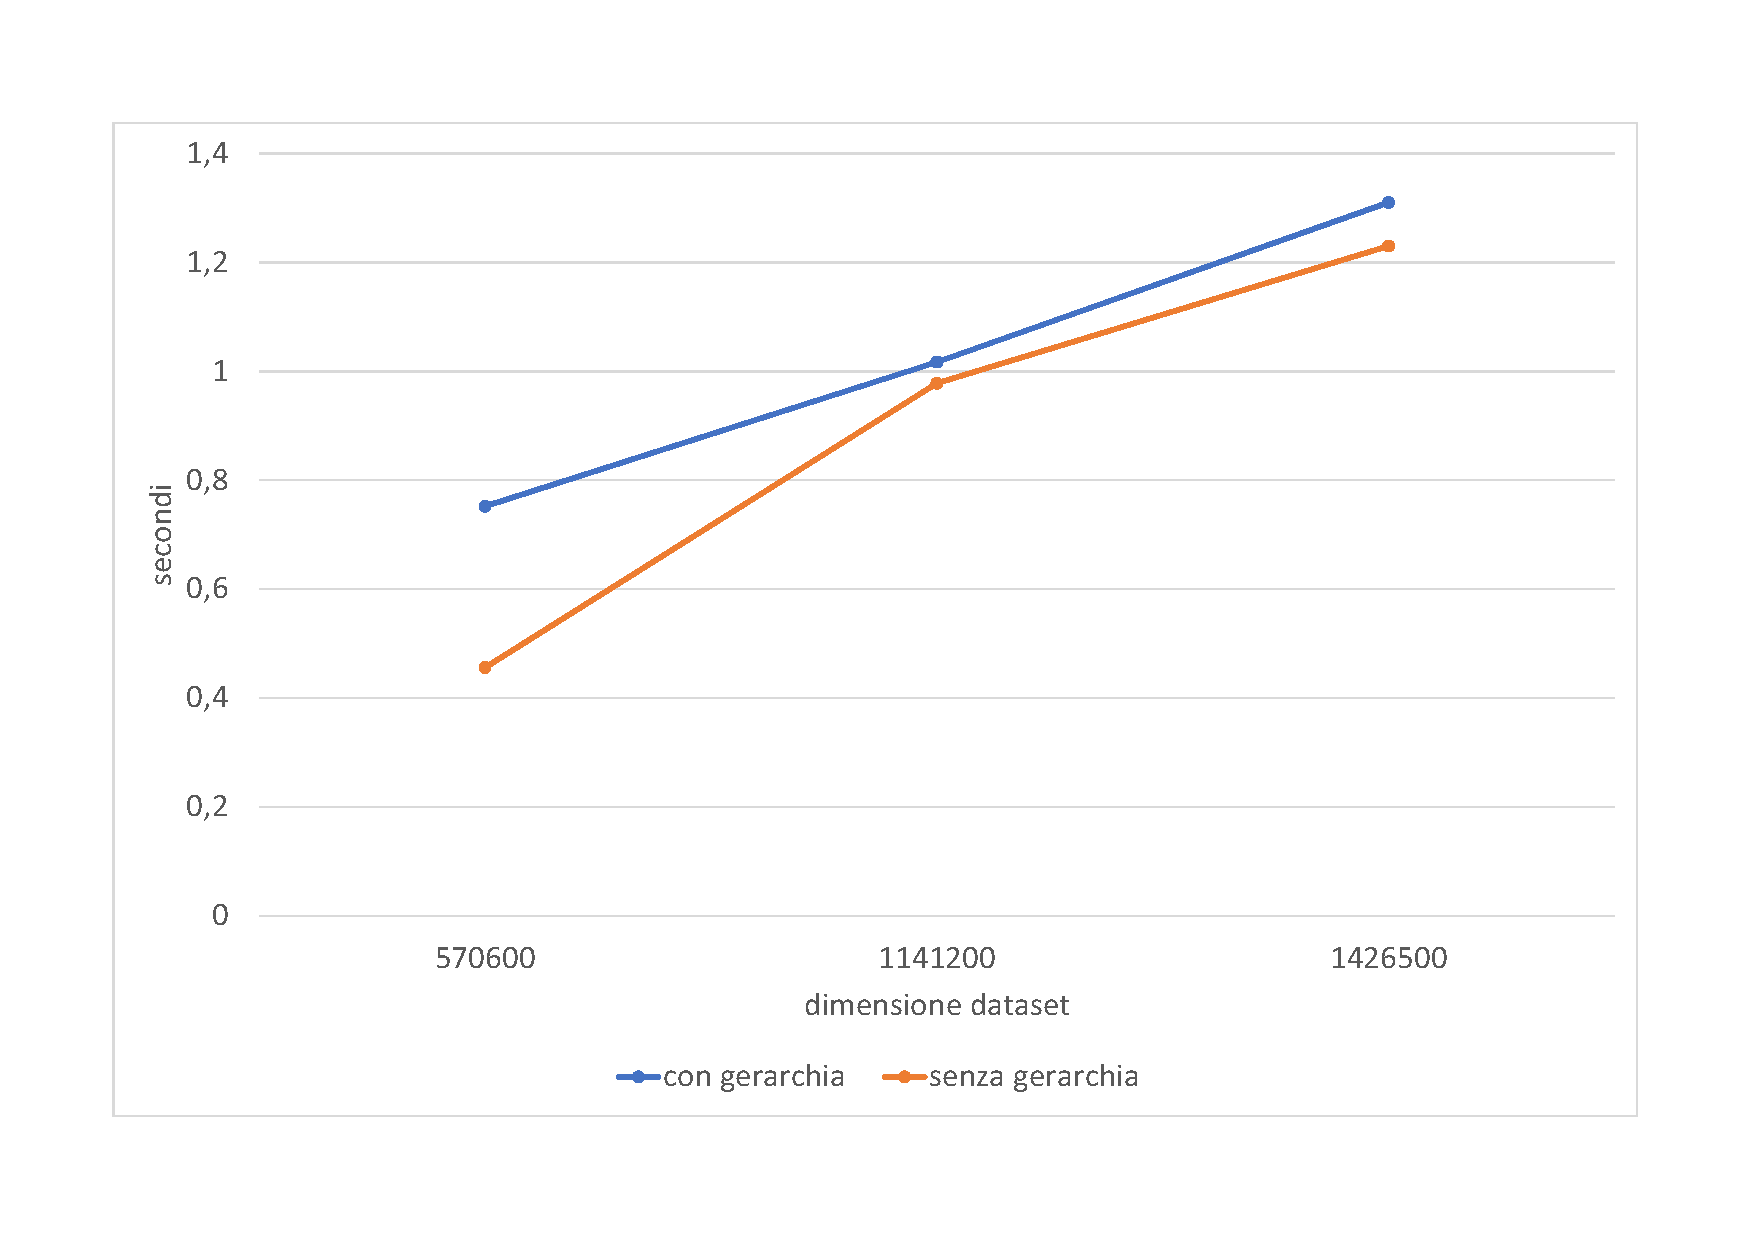
\includegraphics[width=1.0\linewidth]{figures/query_I}
	\caption{Query I - i tempi di calcolo sono molto simili. Tuttavia la formulazione senza gerarchia è più efficiente su qualsiasi dimensione. Ciò è dovuto alla semplicità con cui si può calcolare a run-time il raggruppamento su di un livello di granularità della gerarchia scelta}
	\label{fig:queryi}
\end{figure}
\newpage
\subsection{Query C}
\subsubsection{Consumo medio per intervalli di velocità prefissati}
L'utilizzo della vista materializzata permette di abbattere i tempi di esecuzione della query fino a un trecentesimo: in questo modo il costo di aggiornamento della vista viene immediatamente ammortizzato.
\begin{table}[H]
	\centering
	\begin{tabular}{ccc}
		\rowcolor[HTML]{333333} 
		{\color[HTML]{FFFFFF}Dimensione tab. fatti}
		&
		{\color[HTML]{FFFFFF}Senza vista}
		&
		{\color[HTML]{FFFFFF}Con vista}\\
		\begin{tabular}[c]{@{}l@{}}570.600\end{tabular}              
		& \begin{tabular}[c]{@{}l@{}}0,905s\end{tabular}
		& \begin{tabular}[c]{@{}l@{}}0,020\end{tabular}\\
		\rowcolor[HTML]{C0C0C0}
		\begin{tabular}[c]{@{}l@{}}1.141.200\end{tabular}              
		& \begin{tabular}[c]{@{}l@{}}2,286s\end{tabular}
		& \begin{tabular}[c]{@{}l@{}}0,026s\end{tabular}\\
		\begin{tabular}[c]{@{}l@{}}1.426.500\end{tabular}              
		& \begin{tabular}[c]{@{}l@{}}2,925s\end{tabular}
		& \begin{tabular}[c]{@{}l@{}}0.028s\end{tabular}\\
	\end{tabular}
\caption{Test effettuati su schema non partizionato}
\end{table}
\lstinputlisting[language=mySQL]{./sources/sql/C.sql}
\newpage
\subsection{Query E}
\subsubsection{Efficienza dell'auto per intervalli di RPM}
Si conferma quanto osservato nel caso della query \textbf{C}: utilizzare una vista materializzata permette di abbattere i tempi di esecuzione della query e il costo del refresh risulta ampiamente ammortizzato.
\begin{table}[H]
	\centering
	\begin{tabular}{ccc}
		\rowcolor[HTML]{333333} 
		{\color[HTML]{FFFFFF}Dimensione tab. fatti}
		&
		{\color[HTML]{FFFFFF}Senza vista}
		&
		{\color[HTML]{FFFFFF}Con vista}\\
		\begin{tabular}[c]{@{}l@{}}570.600\end{tabular}              
		& \begin{tabular}[c]{@{}l@{}}0,937s\end{tabular}
		& \begin{tabular}[c]{@{}l@{}}0,018s\end{tabular}\\
		\rowcolor[HTML]{C0C0C0}
		\begin{tabular}[c]{@{}l@{}}1.141.200\end{tabular}              
		& \begin{tabular}[c]{@{}l@{}}2,182s\end{tabular}
		& \begin{tabular}[c]{@{}l@{}}0,028s\end{tabular}\\
		\begin{tabular}[c]{@{}l@{}}1.426.500\end{tabular}              
		& \begin{tabular}[c]{@{}l@{}}2,892s\end{tabular}
		& \begin{tabular}[c]{@{}l@{}}0,030s\end{tabular}\\
		
	\end{tabular}
\caption{Test effettuati su schema non partizionato}
\end{table}
\lstinputlisting[language=mySQL]{./sources/sql/E.sql}
\newpage
\subsection{Query M} \label{sec:m}
\subsubsection{Per ogni test, media di NOx, CO2, Potenza e Velocità}
Questa interrogazione è stata formulata per analizzare le performance del sistema in condizioni sconvenienti. Più precisamente, si intende osservare il calo di prestazioni dovuto all'overhead necessario alla ricostruzione dell'informazione a partire dalle tabelle partizionate. Si intende quindi operare su 4 colonne distribuite su 2 tabelle ottenute dal partizionamento verticale illustrato nella sezione ~\ref{sec:diagrams}.

\subsubsection{Senza partizionamento}
\lstinputlisting[language=mySQL]{./sources/sql/M1.sql}
\subsubsection{Con partizionamento}
\lstinputlisting[language=mySQL]{./sources/sql/M2.sql}
\subsubsection{Esito}
I risultati ottenuti (esposti in figura \ref{fig:querym}) mostrano come un partizionamento ha degli scenari in cui risulta certamente sconveniente, rispetto alla memorizzazione in un'unica tabella. Ciò sottolinea l'importanza della scelta di un buon partizionamento, in fase progettuale, che non prescinde dal set di query che si intende fornire.
\begin{figure}
	\centering
	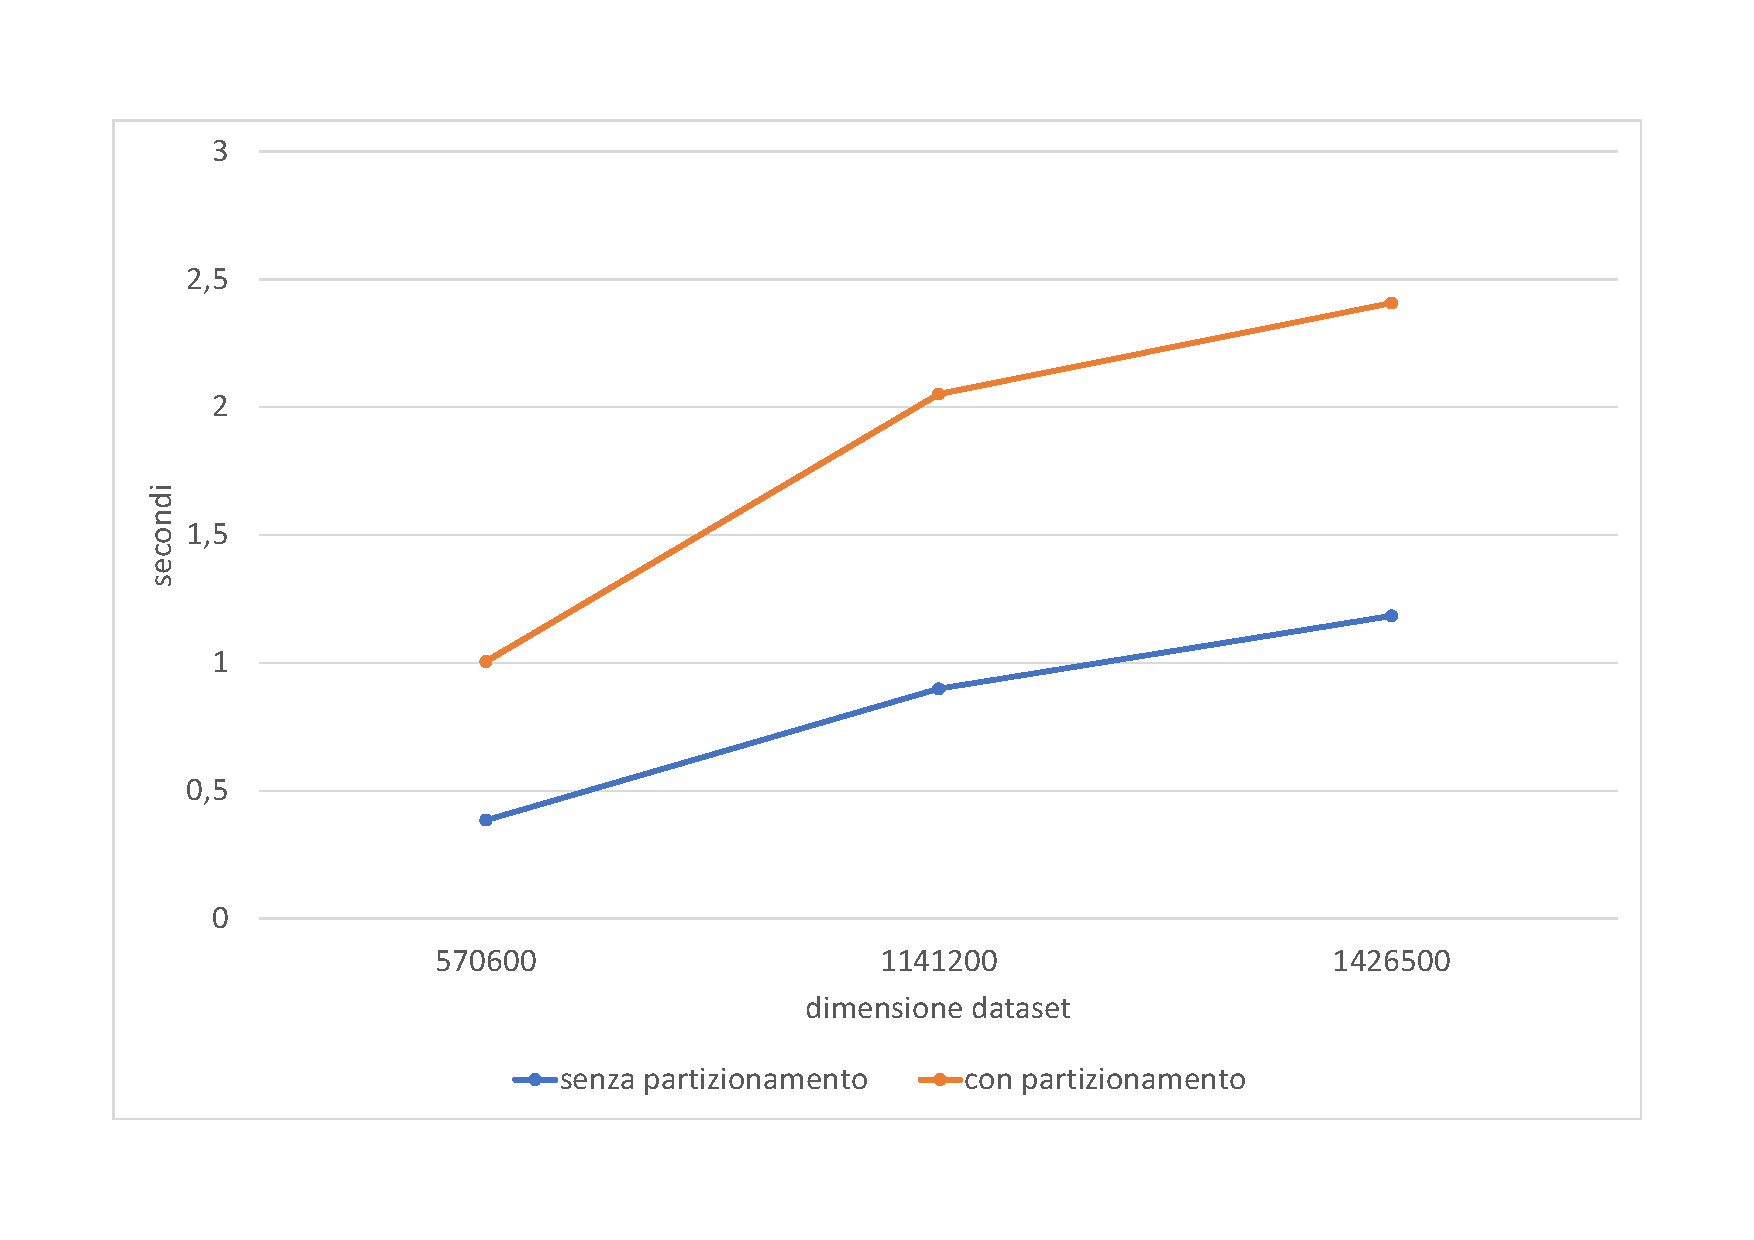
\includegraphics[width=1.0\linewidth]{figures/query_M}
	\caption{Query M - il tempo di ricostruzione dell'informazione attraverso il partizionamento porta al raddoppio del tempo di risposta. Il divario sembra essere costante rispetto alla dimensione del dataset}
	\label{fig:querym}
\end{figure}
\newpage
\subsection{Query T}
\subsubsection{Media e deviazione standard delle temperature}
Inversamente allo scopo della query proposta precedentemente, in questo caso si vuole misurare lo speedup raggiungibile grazie ad un buon partizionamento. Per questo motivo un'interrogazione richiede informazioni di una stessa categoria, memorizzate su di una tabella dedicata alle acquisizioni effettuate dall'Engine Control Unit (ECU), mettendo a confronto i tempi di risposta con un'interrogazione equivalente, che opera sull'intero dataset.
\subsubsection{Interrogazione sull'intero dataset}
\lstinputlisting[language=mySQL]{./sources/sql/T1.sql}
\subsubsection{Interrogazione su tabella ECU}
\lstinputlisting[language=mySQL]{./sources/sql/T2.sql}
\subsubsection{Esito}
Come previsto, le prestazioni ottenute si sono invertite rispetto all'esperimento in \ref{sec:m}. Si ha quindi un notevole risparmio di tempo risolvendo un'interrogazione che richiede informazioni presenti in un'unico partizionamento. 
\begin{figure}
	\centering
	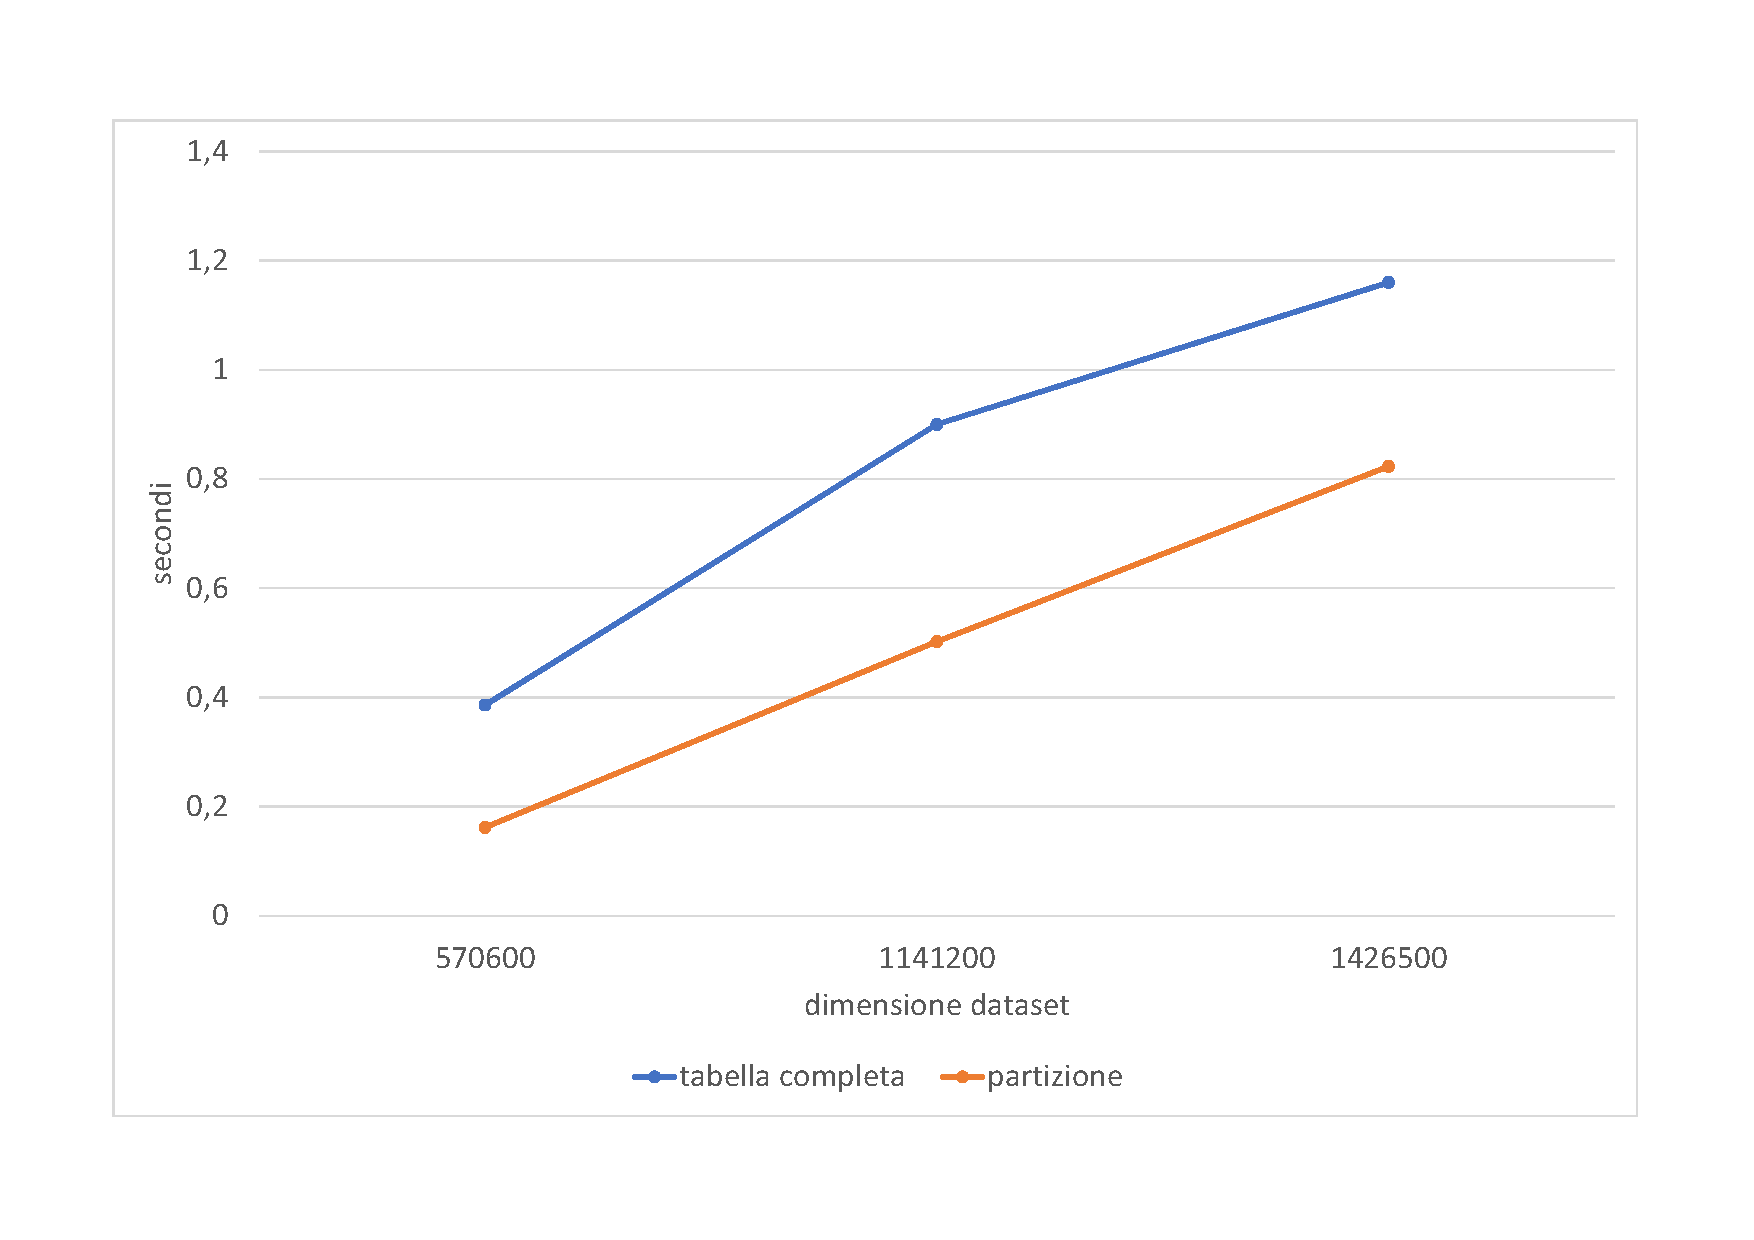
\includegraphics[width=1.0\linewidth]{figures/query_T}
	\caption{Query T - la formulazione che opera sulla partizione risparmia quasi il doppio del tempo grazie al carico minore di dati}
	\label{fig:queryt}
\end{figure}
